% driftwatch - ACL / ARR version (two columns, 8 pages + Limitations + appendix).
% [review] gives the anonymous submission with line numbers; [final] the camera-ready.
\PassOptionsToPackage{table}{xcolor}
\documentclass[11pt]{article}
\usepackage[review]{acl}
\usepackage{times}
\usepackage{latexsym}
\usepackage[T1]{fontenc}
\usepackage[utf8]{inputenc}
\usepackage{microtype}
\usepackage{inconsolata}
\usepackage{graphicx}
\usepackage{booktabs}
\usepackage{multirow}
\usepackage{enumitem}
\usepackage{amsmath,amssymb}
\usepackage{pgfplots}
\pgfplotsset{compat=1.17}

\newcommand{\vone}{\textsc{v1}}
\newcommand{\vtwo}{\textsc{v2}}
\newcommand{\vthree}{\textsc{v3}}

\title{Watching Without Labels: Calibrated Detection of\\Silent Quality Degradation in Deployed Language Models}

\author{Dhruv Parmar \and Pronnati Tapaswi \and Mahak Khurdia \and Aditya Jana \\
  Dhirubhai Ambani University, Gandhinagar, India}

\begin{document}
\maketitle

\begin{abstract}
A language model behind an API can get worse without anyone noticing: the
provider swaps in a smaller model, changes its quantisation, or edits the system
prompt. Production traffic carries no labels, so such changes must be caught from
the answers alone, at a false-alarm rate fixed in advance. We find that the
obvious label-free monitor fails in a specific way: pooled over all traffic, it
alarms in 98--100\% of streams when only the \emph{mix} of user questions changes.
Comparing each task family only with itself, with weights capped by its share,
cuts this to 3.5\% and, on a shift unseen during design, 18.5\%, while four real
faults are still caught in 95.5--99.5\% of streams within about one window and
false alarms stay below the 0.1\% budget. In two pre-registered studies on a
commercial model, the monitor caught the provider's own unannounced update in
93.5\% of streams on benchmark traffic and 89\% on real user requests, although
the update made the model more accurate. Because an alarm means change, not
harm, we add a follow-up that tells the two apart: re-asking the reference model
needs no labels, and grading 100 answers never pointed the wrong way across 2{,}868
alarms. The monitor detects more faults than an embedding MMD test and a 72B LLM
judge on the same streams. It is blind to faults that leave the form of an answer
unchanged.
\end{abstract}

\section{Introduction}

Teams that build on hosted language models depend on a component they cannot
inspect. The model behind an endpoint may be replaced by a cheaper one, served at a
lower precision, or wrapped in a different system prompt, and nobody downstream is
told. Users then see worse answers before engineers see anything at all.
Longitudinal measurements of commercial models have documented exactly this kind of
silent behaviour change~\citep{chen2023chatgpt}. The usual remedy, a labelled
evaluation set run on a schedule, is slow and expensive. It also measures a fixed
benchmark rather than the traffic that actually matters.

We ask whether \emph{a monitor that sees only the model's answers to live traffic,
with no labels, can raise an alarm when quality drops, at a false-alarm rate fixed
before deployment}. This is harder than generic drift
detection~\citep{gama2014survey,rabanser2019failing} for one reason above all:
user traffic changes on its own. A week of maths homework looks different from a
week of trivia, and a monitor that flags every change of topic is switched off.
Five research questions follow.
\begin{enumerate}[label=\textbf{RQ\arabic*}, leftmargin=*]
  \item \textbf{Calibrated alarms.} Does the monitor keep, on healthy traffic, the
  false-alarm rate it was calibrated to?
  \item \textbf{Real faults.} Does it detect actual model swaps and prompt edits,
  not injected noise, and how soon after the onset?
  \item \textbf{Degradation or a change of topic.} Does it stay quiet when only the
  mix of questions changes?
  \item \textbf{Transfer.} Do RQ1--RQ3 hold for deployed models of other
  families, recalibrated with nothing tuned?
  \item \textbf{A real deployment.} Does it notice an update that a provider
  actually shipped, unannounced, and on real user requests?
\end{enumerate}
RQ1--RQ3 are answered in \S\ref{sec:results}, their limits in
\S\ref{sec:robust}, RQ4 in \S\ref{sec:transfer} and RQ5 in \S\ref{sec:api}.

\paragraph{Contributions}
\begin{itemize}
  \item \textbf{A failure of the obvious design, and a fix.} Pooled label-free
  statistics mostly measure \emph{which kinds} of question a window holds, so a
  pooled monitor mistakes a change of topic for degradation. Per-slice scoring
  with capped weights removes most of this, judged on a shift unseen during
  design and on 50 random mixtures (\S\ref{sec:scoring}, \S\ref{sec:results}).
  \item \textbf{A real, unannounced update, caught.} Two pre-registered studies on
  a commercial model: the provider's own update is detected within one window
  on benchmark traffic and three on real user traffic, and a 4-bit build whose answers
  did not change is not (\S\ref{sec:api}, Appendix~\ref{app:chat}).
  \item \textbf{From alarm to action.} Since the update improved accuracy, an
  alarm must be triaged. A label-free readout and a small graded check separate
  harm from harmless change and never point the wrong way
  (\S\ref{sec:discussion}, Appendix~\ref{app:triage}).
  \item \textbf{A strong baseline beaten, and limits mapped.} Under the same
  calibration, the monitor detects more faults than embedding MMD and
  reference-free LLM judges at 14B and 72B, which grade style rather than
  correctness. Dose, single-slice faults and transfer to four other models show
  where it fails (\S\ref{sec:robust}).
  \item \textbf{A protocol.} Thresholds are frozen before any fault answer is
  read, every analysis verifies the frozen record, and the false-alarm guarantee
  and its assumptions are stated (Appendix~\ref{app:guarantee}). Code and records
  are released.
\end{itemize}

\section{Related work}

\paragraph{Dataset and concept drift}
Drift detection has a long history in streaming learning~\citep{gama2014survey}.
\citet{rabanser2019failing} compare two-sample tests on learned representations
for detecting covariate shift, and \citet{lipton2018detecting} detect label shift
from a black-box predictor's outputs. These methods ask whether the
\emph{inputs} changed. We ask whether the \emph{model} changed, and we treat a
change in the inputs alone as a false alarm. This inversion drives our
per-slice design.

\paragraph{Sequential change detection}
CUSUM~\citep{page1954continuous} and the Page--Hinkley
test~\citep{hinkley1971inference} accumulate evidence across observations to find
small persistent shifts. We use fixed-window thresholds as the primary monitor
because their false-alarm rate per window is directly interpretable. We compare
both sequential tests on the same statistics in \S\ref{sec:seq}.

\paragraph{Kernel two-sample tests}
The maximum mean discrepancy~\citep{gretton2012kernel} is a natural label-free
baseline on sentence embeddings. We include it and find that it is sensitive to
model faults but cannot tell them apart from harmless shifts.

\paragraph{LLM-as-a-judge}
A strong model grading answers agrees well with human preferences, but it favours
longer answers and grades maths and reasoning poorly~\citep{zheng2023judging}.
A judge is the obvious alternative to a label-free monitor, at the cost of one
more inference per answer. We run one as a baseline under our calibration and
find that it inherits exactly these biases as a monitor.

\paragraph{Consistency as a quality signal}
Agreement among sampled answers predicts correctness: self-consistency improves
reasoning accuracy~\citep{wang2023selfconsistency}, and SelfCheckGPT uses sample
disagreement to flag hallucinations~\citep{manakul2023selfcheckgpt}. We use
agreement not to judge single answers but as a population statistic whose
distribution shifts when the model behind it changes.

\paragraph{Behaviour change in deployed models}
\citet{chen2023chatgpt} show that the behaviour of commercial models changed
substantially across versions over a few months. Our work offers a way
to notice such changes from traffic, without rerunning a benchmark.

\section{Method}
\label{sec:method}

\subsection{Setting}
A deployed model $M$ answers a stream of queries. The monitor sees each query's
task family (slice) and $k=4$ answers sampled at temperature 0.7 with distinct
seeds. It sees no labels. Queries are grouped into overlapping windows of $W=200$
queries with stride $S=50$, so a new window closes every 50 queries. A window's
standard composition across the seven slices is fixed
(Table~\ref{tab:corpus}). Before deployment, the operator has healthy answers on a
calibration set and chooses a family-wise false-alarm budget $\beta$ per window;
we use $\beta=10^{-3}$.

\subsection{Signals}
Each signal maps a window to a scalar score that is larger when the window is
further from healthy.
\begin{description}
  \item[S1 length.] The two-sample Kolmogorov--Smirnov statistic between answer
  lengths (whitespace tokens) in the window and in the healthy reference. A failed
  parse has length zero.
  \item[S3 self-consistency.] For each query, the mean pairwise agreement among
  its $k$ answers. Agreement is exact match after canonicalisation for verifiable
  slices and word-set Jaccard overlap otherwise; a failed parse agrees with
  nothing. The score is the shift of the window mean from the reference.
  \item[S4 lexical diversity.] The moving-average type--token
  ratio~\citep{covington2010mattr} over 25-token windows, together with the
  trigram repetition rate.
  \item[S6 label entropy.] The Miller--Madow-corrected entropy of predicted
  intents on the banking77 slice. A collapse onto a few labels lowers it.
  \item[S7 embedding shift.] The centroid shift and change in dispersion of
  answer embeddings from Nomic Embed v1.5~\citep{nussbaum2024nomic},
  relative to the healthy reference cloud.
\end{description}
Refusal rate (S2) and JSON validity (S5) were implemented but left unmonitored:
the healthy model essentially never refused or broke the JSON format, so both
were constant on calibration data and had no threshold to fit.

\subsection{Calibration}
For each signal we draw 20{,}000 bootstrap windows of standard composition from
the healthy calibration answers and score them. With $m=5$ signals, the per-signal
level is the Šidák~\citep{sidak1967rectangular} split of the family-wise budget,
\[
  \alpha' = 1-(1-\beta)^{1/m} \approx 2.0\times10^{-4},
\]
so the threshold is the $1-\alpha'$ quantile of the bootstrap scores. This quantile
lies beyond all but about four of the 20{,}000 draws, so we estimate it with a
peaks-over-threshold fit of a generalised Pareto distribution to the upper
tail~\citep{pickands1975statistical}. The plain empirical quantile is used only
when the tail holds enough draws. A window alarms if any signal crosses its
threshold; Appendix~\ref{app:guarantee} states what this guarantees and under which
assumptions. Thresholds, signal list, scoring version and data hashes are written to
a \emph{frozen record}. Every later analysis verifies the record and refuses to run
on any mismatch.

\subsection{Pooled versus per-slice scoring}
\label{sec:scoring}
\paragraph{\vone: pooled} Each window is compared with one healthy reference
pooled over all slices. A window heavy in long-form slices therefore looks
``longer'' and ``semantically elsewhere'' even when every answer in it is healthy.

\paragraph{\vtwo: per slice} Each signal is fitted once per slice on that slice's
healthy answers. A window is scored slice by slice, and the slice scores are
averaged with the standard window weights, renormalised over the slices present.
S6 compares a window's entropy with the healthy entropy distribution \emph{at the
same number of banking77 queries}, because entropy over 77 labels depends on
sample size.

\paragraph{\vthree: per slice, capped} \vtwo{} gives a thin slice its full weight
even though its score is far noisier. \vthree{} weights slice $s$ by
$w_s=\min(n_s, q_s)$, where $n_s$ is its count in the window and $q_s$ its
standard quota. On every standard window this equals \vtwo.

\vone{}'s thresholds depend on the healthy calibration answers alone, whose hash
every analysis checks. The fault rounds predate the freeze by hours; the one later
choice, dropping two signals, was forced: both are constant on healthy data. \vtwo{} and \vthree{} were
designed \emph{after} seeing \vone{} alarm on the first harmless shift (F4), so
F4 cannot judge them fairly. Both were frozen before a second, opposite harmless
shift (F6) was generated, and F6 is the test that counts.

\section{Experimental setup}
\label{sec:setup}

\paragraph{Corpus}
We build 5{,}000 queries over seven slices (Table~\ref{tab:corpus}): grade-school
maths~\citep{cobbe2021gsm8k}, open-domain trivia~\citep{joshi2017triviaqa},
reading comprehension with unanswerable questions~\citep{rajpurkar2018squad2},
intent classification~\citep{casanueva2020banking77}, extreme
summarisation~\citep{narayan2018xsum}, long-form explanations~\citep{fan2019eli5},
and \textsf{jsonx}, a structured-extraction task we synthesised from a fixed JSON
schema. The queries are split into calibration (2{,}500), held-out (1{,}000) and
fault (1{,}500) sets. No query or prompt appears in two splits. The only shared
material is SQuAD passages (24--25\%) and \textsf{jsonx} item titles. Thresholds
are fitted on answer statistics, never on answers to look up.

\begin{table*}[t]
  \centering\small
  \caption{Slices, their standard share of a 200-query window, and the healthy
  model's oracle accuracy on the fault questions. Accuracy is used only for
  evaluation, never by the monitor.}
  \label{tab:corpus}
  \begin{tabular}{lrrl}
    \toprule
    slice & quota / 200 & healthy acc. & oracle \\
    \midrule
    gsm8k & 28 & 0.956 & final number \\
    triviaqa & 28 & 0.570 & alias match \\
    squad2 & 28 & 0.823 & span / abstain \\
    banking77 & 20 & 0.743 & label \\
    jsonx & 8 & 0.538$^\ast$ & exact JSON \\
    xsum & 44 & -- & -- \\
    eli5 & 44 & -- & -- \\
    \bottomrule
  \end{tabular}\\[2pt]
  {\footnotesize $^\ast$Strict key; 97.9\% when a priority off by one is accepted.
  Left out of mean accuracy.}
\end{table*}

\paragraph{Models and conditions}
All models are served locally with Ollama at Q4\_K\_M quantisation; the digest of
every build is pinned and recorded on every answer. The healthy model is
\texttt{gemma4:26b-a4b}, a mixture-of-experts model with about 4B active
parameters. Table~\ref{tab:conditions} lists the conditions. The faulty models
were chosen to be measurably worse. On a 500-query pilot, the step from F2 to F1
was $+7.2$ points (95\% CI $[3.0, 11.4]$), and a dense 12B sibling was rejected
because it was \emph{not} distinguishable from the healthy model. F3 keeps the
healthy model and adds two plausible lines to the system prompt: a terseness
instruction and hedging on uncertain questions. Its text was fixed before the
fault round was generated. F4 and F6 replay \emph{healthy} answers with a shifted
question mix (total-variation distance 0.26 and 0.41 from the standard mix): F4
leans towards long-form slices, F6 towards short ones. F7 reruns the healthy
model on fresh seeds and is a negative control. In total there are 64{,}000
answers across seven generation rounds.

\begin{table*}[t]
  \centering\small
  \caption{Conditions. Accuracy is the oracle mean on the 1{,}500 fault questions,
  with \textsf{jsonx} excluded.}
  \label{tab:conditions}
  \begin{tabular}{llrl}
    \toprule
    id & change & accuracy & should alarm? \\
    \midrule
    healthy & \texttt{gemma4:26b-a4b} & 0.773 & -- \\
    F1 & smallest sibling, \texttt{gemma4:e2b} & 0.593 & yes \\
    F2 & small sibling, \texttt{gemma4:e4b} & 0.666 & yes \\
    F3 & edited system prompt, healthy model & 0.745 & yes \\
    F5 & older generation, \texttt{gemma3:12b} & 0.732 & yes \\
    F4 & healthy answers, long-form-heavy mix & 0.773 & no \\
    F6 & healthy answers, short-form-heavy mix & 0.773 & no \\
    F7 & healthy model, fresh seeds & 0.773 & no \\
    \bottomrule
  \end{tabular}
\end{table*}

\paragraph{Replay protocol}
Each run builds a stream of 40 windows. The stream begins with healthy answers to
fault questions. At an onset drawn at window 10 or later, the stream switches to
the condition's answers to the \emph{same} questions, so the question
distribution does not change at the onset; for F4 and F6 only the mix changes.
We run 200 streams per condition. We report the detection rate with Wilson 95\%
intervals~\citep{wilson1927probable}, the latency in windows from the first window
containing any faulty query, the false-alarm rate on healthy windows before the
onset, and alarms on the 17 real held-out windows. A latency of 1 means the alarm
came 50 queries after the onset window.

\section{Results}
\label{sec:results}

\begin{table*}[t]
  \centering\small
  \caption{Main result: runs alarmed out of 200 (Wilson 95\% interval) and median
  latency in windows. The last rows give false-alarm rates on healthy windows before
  the onset (all conditions) and on the 17 real held-out windows (budget 0.1\%).}
  \label{tab:main}
  \setlength{\tabcolsep}{5pt}
  \begin{tabular}{lccc}
    \toprule
    condition & \vone{} pooled & \vtwo{} per slice & \vthree{} per slice, capped \\
    \midrule
    F1 e2b & 196 (95--99\%), 1 & 198 (96--100\%), 1 & 198 (96--100\%), 1 \\
    F2 e4b & 197 (96--99\%), 1 & 197 (96--99\%), 1 & 197 (96--99\%), 1 \\
    F3 prompt & 200 (98--100\%), 0 & 199 (97--100\%), 0 & 199 (97--100\%), 0 \\
    F5 gemma3 & 192 (92--98\%), 1 & 191 (92--98\%), 1 & 191 (92--98\%), 1 \\
    \midrule
    F4 mix (seen) & \textbf{196} (95--99\%), 1 & 48 (19--30\%), 8 & 7 (2--7\%), 5 \\
    F6 mix (unseen) & \textbf{200} (98--100\%), 0 & 190 (91--97\%), 3 & 37 (14--24\%), 12 \\
    F7 fresh seeds & 4 (1--5\%), 12 & 0 (0--2\%) & 0 (0--2\%) \\
    \midrule
    pre-onset false alarms & 0.076\% & 0.017\% & 0.017\% \\
    held-out windows & 0/17 & 0/17 & 0/17 \\
    \bottomrule
  \end{tabular}
\end{table*}

\paragraph{Real faults are caught quickly (RQ2)}
Under every scoring, the four real faults are detected in 95.5--100\% of streams
(Table~\ref{tab:main}). The median latency is one window, meaning the alarm comes
within 50 queries of the first faulty answer. F3, the prompt edit, is caught at
the onset window itself. Its accuracy cost is only 2.8 points, but it shortens
answers sharply. The fresh-seed control F7 almost never alarms. Its four \vone{}
alarms come late in the stream (median window 12), consistent with chance.

\paragraph{The pooled monitor cannot tell degradation from a change of topic (RQ3)}
\vone{} alarms on F4 in 98\% of streams and on F6 in 100\%, although every answer
in those streams is healthy. Over 50 random harmless mixtures, its mean alarm rate
is 93.9\%. Pooled length and embedding statistics mostly measure \emph{which
slices} a window contains.

\paragraph{Capped per-slice scoring fixes most of this (RQ3)}
\vtwo{} removes most F4 alarms (24\%) but still alarms on the unseen F6 in 95\% of
streams. The cause is thin slices: a slice with 10 queries counts as much as one
with 28. \vthree{} caps the weights and brings F6 down to 18.5\% and F4 to 3.5\%,
with detection of the real faults unchanged. Over 50 random mixtures, \vthree{}
alarms in 4.8\% of streams on average (median 1.0\%). Only one mixture in fifty
alarms in more than half its streams. The alarm rate rises with shift size
(Spearman $\rho=0.65$): it is at most 1.3\% for total-variation distances up to
0.3, 8.1\% between 0.3 and 0.4, and 26\% above 0.4. Large, sudden changes of topic remain visible, which an
operator may well want.

\paragraph{False alarms stay within budget (RQ1)}
Pre-onset false alarms under \vthree{} run at 0.017\%, against a budget of 0.1\%.
The thresholds come from one bootstrap seed, so we recalibrated with ten: the
rate stays at 0.017--0.041\%, thresholds move by 5--15\%, and detection of F1--F5
by at most one point (Appendix~\ref{app:seeds}). \vone{} is less stable
(0.076--0.253\%; the frozen seed gives the lowest).
Questions are a finite sample, so we also resample them. Over 50 stratified
half-samples of the fault questions, the 95\% interval for the pre-onset rate is
0--0.061\%, still under budget. The detection intervals from half-sampling agree
with the Wilson intervals to within a point (Appendix~\ref{app:half}).

\paragraph{Which signals carry the result}
Table~\ref{tab:ablation} shows single-signal configurations, each calibrated to the
same family-wise budget. Length alone (S1) catches every real fault and almost
none of the harmless shifts under \vthree{}. Removing it costs most of the F5
detection (95.5\%$\to$40.5\%). Self-consistency (S3) and lexical diversity (S4)
catch the sibling faults but at most 68\% of F3 and half of F5. They still matter:
\S\ref{sec:lengthmatched} shows that when mean answer length is matched, either
alone still catches 82--97\% of streams. Two baselines are instructive. A mean-length threshold
detects F2--F5 but alarms on every harmless shift. Without the Šidák correction,
F6 alarms rise to 44.5\% and F7 to 4\%.

\begin{table*}[t]
  \centering\small
  \caption{Ablation under \vthree{} (\% of 200 runs alarmed). Every row is
  recalibrated to the same family-wise budget except ``no Šidák''. The LLM
  judges grade every answer with Qwen 2.5 at 14B or 72B (\S\ref{sec:judge}).}
  \label{tab:ablation}
  \setlength{\tabcolsep}{4.5pt}
  \begin{tabular}{lrrrr|rrr|r}
    \toprule
    configuration & F1 & F2 & F3 & F5 & F4 & F6 & F7 & pre-onset \\
    \midrule
    all five signals & 99.0 & 98.5 & 99.5 & 95.5 & 3.5 & 18.5 & 0.0 & 0.017\% \\
    without S1 length & 98.0 & 98.5 & 87.0 & 40.5 & 4.0 & 20.0 & 0.5 & 0.026\% \\
    only S1 length & 98.5 & 97.0 & 100.0 & 97.0 & 0.0 & 1.0 & 1.0 & 0.029\% \\
    only S3 consistency & 98.0 & 98.5 & 68.0 & 23.0 & 2.5 & 1.5 & 2.0 & 0.079\% \\
    only S4 lexical & 97.0 & 89.0 & 0.0 & 51.5 & 0.0 & 21.5 & 0.5 & 0.009\% \\
    only S7 embedding & 91.5 & 26.0 & 88.5 & 40.0 & 6.0 & 30.0 & 0.5 & 0.058\% \\
    \midrule
    mean-length baseline & 71.0 & 95.5 & 100.0 & 97.5 & 100.0 & 100.0 & 1.0 & 0.198\% \\
    no Šidák & 99.0 & 98.5 & 100.0 & 97.0 & 9.0 & 44.5 & 4.0 & 0.175\% \\
    embedding MMD & 97.5 & 87.5 & 92.5 & 83.5 & 99.0 & 98.0 & 7.5 & 0.524\% \\
    LLM judge, 14B & 93.0 & 49.5 & 91.0 & 5.5 & 4.5 & 18.0 & 6.0 & 0.437\% \\
    LLM judge, 72B & 98.5 & 90.5 & 92.0 & 58.5 & 1.5 & 8.5 & 0.0 & 0.061\% \\
    \bottomrule
  \end{tabular}
\end{table*}

\paragraph{An MMD baseline detects change, not degradation}
An unbiased RBF-kernel MMD$^2$~\citep{gretton2012kernel} is computed on per-question
mean embeddings against 500 calibration questions, with a median-heuristic
bandwidth and the same budget. It catches 83.5--97.5\% of real faults, but also
98--99\% of harmless shifts, and its pre-onset rate is five times the budget.
Paired with the monitor on the same streams, it misses 22, 14 and 24 more F2, F3
and F5 streams ($p\le 1.2\times10^{-4}$) and alarms on 191 and 159 more F4 and F6
streams. A
two-sample test on embeddings answers ``did the traffic change?'', which is not
the question we need answered.

\begin{figure}[t]
  \centering
  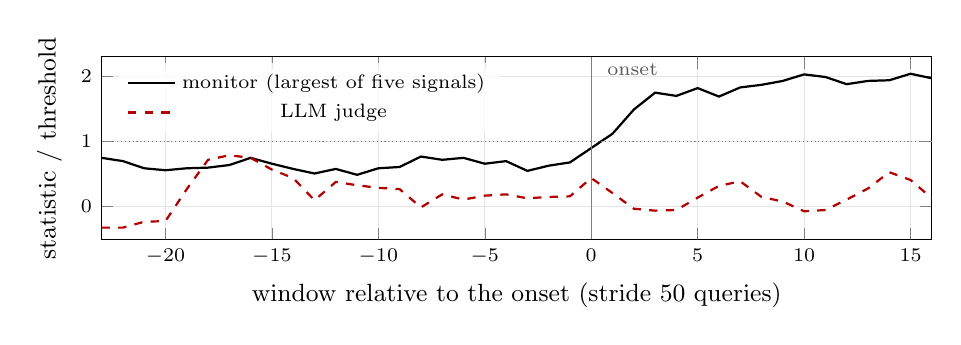
\begin{tikzpicture}
    \begin{axis}[
      width=\columnwidth, height=3.9cm,
      xlabel={window relative to the onset (stride 50 queries)},
      ylabel={statistic / threshold},
      xmin=-23, xmax=16, ymin=-0.5, ymax=2.3, grid=major, grid style={gray!20},
      legend style={font=\scriptsize, at={(0.02,0.97)}, anchor=north west, draw=none, fill=white, fill opacity=0.8, text opacity=1},
      tick label style={font=\scriptsize}, label style={font=\small},
    ]
      \addplot[thick, black] coordinates {(-23,0.75) (-22,0.70) (-21,0.59) (-20,0.56) (-19,0.59) (-18,0.60) (-17,0.64) (-16,0.75) (-15,0.66) (-14,0.58) (-13,0.51) (-12,0.58) (-11,0.49) (-10,0.59) (-9,0.61) (-8,0.77) (-7,0.72) (-6,0.75) (-5,0.66) (-4,0.70) (-3,0.55) (-2,0.63) (-1,0.68) (0,0.90) (1,1.12) (2,1.49) (3,1.75) (4,1.70) (5,1.82) (6,1.69) (7,1.83) (8,1.87) (9,1.93) (10,2.03) (11,1.99) (12,1.88) (13,1.93) (14,1.94) (15,2.04) (16,1.97)};
      \addlegendentry{monitor (largest of five signals)}
      \addplot[thick, red!70!black, dashed] coordinates {(-23,-0.32) (-22,-0.32) (-21,-0.23) (-20,-0.22) (-19,0.27) (-18,0.72) (-17,0.79) (-16,0.75) (-15,0.57) (-14,0.44) (-13,0.10) (-12,0.38) (-11,0.33) (-10,0.29) (-9,0.27) (-8,-0.01) (-7,0.19) (-6,0.11) (-5,0.17) (-4,0.19) (-3,0.13) (-2,0.15) (-1,0.16) (0,0.44) (1,0.21) (2,-0.03) (3,-0.06) (4,-0.05) (5,0.14) (6,0.32) (7,0.39) (8,0.15) (9,0.08) (10,-0.07) (11,-0.05) (12,0.11) (13,0.28) (14,0.53) (15,0.41) (16,0.13)};
      \addlegendentry{LLM judge}
      \addplot[gray, densely dotted, forget plot] coordinates {(-23,1) (16,1)};
      \draw[gray] (axis cs:0,-0.5) -- (axis cs:0,2.3);
      \node[anchor=west, font=\scriptsize, gray!70!black] at (axis cs:0.3,2.1) {onset};
    \end{axis}
  \end{tikzpicture}
  \caption{One replayed F5 stream under \vthree{} (the first of 200). Each line is
  its alarm statistic divided by its threshold, so an alarm is a value above 1. The
  monitor crosses one window after the onset, driven by S1 length; the judge never
  does. The same stream, thresholds and budget apply to both.}
  \label{fig:stream}
\end{figure}

\paragraph{An LLM judge grades style, not correctness}
\label{sec:judge}
A second model grades every answer from 1 to 10, reference-free: it sees the
request and the answer, never the ground truth or the system prompt. The judge is
\texttt{qwen2.5:14b} at temperature 0, from a family that none of the graded
models belong to. The prompt, parse rule and window statistic (healthy mean grade
minus the window's, one-sided) were fixed and committed before any grade was read.
It graded all 50{,}000 answers of the healthy model, F1--F3, F5 and F7; 18 replies
held no grade and are counted, not dropped. Thresholded and replayed exactly like
the other rows, the judge catches F1 (93.0\%) and F3 (91.0\%) but only 49.5\% of
F2 streams and 5.5\% of F5, against 98.5\% and 95.5\% for the monitor, and its
pre-onset rate is 4.4 times the budget. The mean grades show why. Against the
healthy answers to the same questions, the prompt edit F3 costs 1.80 points on
\textsf{eli5} and 0.77 on \textsf{gsm8k}, because it changes length and style. The
weaker siblings lose up to 1.68 points on \textsf{triviaqa}, where the judge can
check a fact itself, but on \textsf{gsm8k} they score \emph{higher} than the healthy
model, and F5 gains 0.04 overall. The judge sees a weaker model only where it can
check the answer without a reference (Appendix~\ref{app:judge};
Figure~\ref{fig:stream} shows one F5 stream). Paired on the same streams with an
exact McNemar test, the monitor alarms on every fault stream the judge alarms on,
and on 12, 98, 17 and 180 more for F1, F2, F3 and F5 ($p\le 5\times10^{-4}$); the
judge adds 12 false alarms on F7 ($p=5\times10^{-4}$). Holding the judge to the
budget would only raise its threshold and lower its detection further.

A larger judge closes part of the gap. We pre-registered a second version that
changes only the judge, to Qwen 2.5 72B (same family, five times larger, fp8 on a
hosted GPU), and graded the same 50{,}000 answers. It catches F2 in 90.5\% of
streams and F5 in 58.5\%, stays within budget before the onset (0.061\%) and never
alarms on F7; under \vthree{} it also alarms on F6 less than the monitor (8.5\%
against 18.5\%). Paired on the same streams, the monitor still catches 16, 15 and
74 more F2, F3 and F5 streams ($p\le 6\times10^{-5}$), while the judge alarms on
20 fewer F6 streams (31 against 11, $p=0.003$). The larger judge is a strong
baseline, but it misses two in five streams of the older-generation model, and it
needs a 72B call for every answer (\$6.81 for these grades).

\begin{table*}[t]
  \centering\small
  \caption{The hosted-API study: runs alarmed out of 200 and median latency in
  windows, with frozen thresholds. Accuracy changes are against the healthy answers
  to the same questions, on the four scored slices.}
  \label{tab:api}
  \setlength{\tabcolsep}{5pt}
  \begin{tabular}{llcc}
    \toprule
    condition & what changed & \vone{} pooled & \vthree{} capped \\
    \midrule
    U1 & DeepSeek's update; accuracy $+0.2$ to $+8.6$ & 182 (91.0\%), 2 & 187 (93.5\%), 1 \\
    Q1 & 4-bit host; accuracy within $\pm1.5$ & 4 (2.0\%) & 2 (1.0\%) \\
    \midrule
    F4 mix (seen) & question mix only & 198 (99.0\%) & 17 (8.5\%) \\
    F6 mix (unseen) & question mix only & 200 (100\%) & 58 (29.0\%) \\
    F7 fresh seeds & nothing & 3 (1.5\%) & 3 (1.5\%) \\
    \midrule
    pre-onset false alarms & & 0.092\% & 0.129\% \\
    held-out windows & & 0/17 & 0/17 \\
    \bottomrule
  \end{tabular}
\end{table*}

\section{Robustness and limits}
\label{sec:robust}

\subsection{Removing the length shortcut}
\label{sec:lengthmatched}
A smaller model writes shorter answers, so a skeptic may suspect that the monitor
is just a length detector. For each slice, we keep the 50\% of fault questions
whose faulty answers are closest in length to the healthy ones. This brings the
length ratio to $0.95$ (F1) and $0.90$ (F2) while the accuracy drop remains
10.0 and 7.4 points. Detection stays at 99.5\% and 98\% (S1 still sees the shape of the length
distribution); S3 alone fires in 82--94\% of runs and S4 in 86--97\%. Pre-onset
false alarms on these restricted sets rise to 0.8--2.3\% per window, enough for
at most 11--30\% of the detections.

\subsection{Partial and gradual degradation}
\label{sec:seq}
In practice, a fault may affect only part of the traffic (for example, a
canary deployment) or arrive gradually. We mix a dose $d$ of faulty answers into
the post-onset stream, or ramp it from 0 to 100\% over 30 windows
(Appendix~\ref{app:dose}, Figure~\ref{fig:dose}). The threshold monitor reliably catches doses of 25\% and
above, including the ramp. At 10\% it catches only 17.5--21\%, and at 5\% almost
nothing. On the same statistics, standardised on healthy calibration streams, we
set CUSUM~\citep{page1954continuous} and
Page--Hinkley~\citep{hinkley1971inference} to the same per-signal alarm rate per
window. Page--Hinkley detects 53--57\% at a 10\% dose and 15--23\% at 5\%, while
staying within budget before the onset (0.00--0.06\%). CUSUM catches 99.5\% at 10\%
but fires on F7 in 17.5\% of streams. Its pre-onset false-alarm rate is 3--6 times
the budget, because evaluation streams sit $+0.64$ standard deviations from
calibration on S7, and CUSUM accumulates this offset. Page--Hinkley is the better
companion; CUSUM needs a recalibrated reference before it is safe.



\subsection{Faults confined to one slice}
\label{sec:slice}
If only one kind of question is routed to a bad model, the fault occupies 4--22\%
of each window. Under \vthree{}, detection follows how visible the change is in
that slice, not how large the accuracy drop is. Faults on long-form eli5 are
caught in 95--97\% of streams and on gsm8k in 86--91\% (F1, F2), through length and
lexical change. Triviaqa reaches 48--78\% and squad2 34--67\%. Banking77 and
\textsf{jsonx} are blind spots ($\le$3.5\%) even when the accuracy drop is 9.7
points: a wrong intent label looks just like a right one. A label-free monitor
cannot see a fault that does not change the surface of the answers. This is the
clearest limit of our approach.

\subsection{One answer, calibration and window size}
\label{sec:oneanswer}
With one answer per query (no S3, a quarter of the cost), \vthree{} still catches
94--98.5\% of real faults at 0.047\% pre-onset false alarms; \vone{} does not
(0.65\%). Thresholds move under 9\% from half the calibration questions up, though F6
alarms vary across draws, and larger windows help at small doses (Appendix~\ref{app:sens}).

\subsection{Other healthy models (RQ4)}
\label{sec:transfer}
Every result above treats one model as the deployment. To test transfer, we
rerun the whole method with four other models as the healthy deployment, each on
all 5{,}000 questions: \texttt{gemma3:12b} (an older Gemma generation) and three
families from other vendors, \texttt{qwen2.5:14b}, \texttt{llama3.1:8b} and
\texttt{phi4:14b}. The gemma3 round is part of the 64{,}000 answers above; the
three others add 60{,}000 answers in three more rounds. For each deployment
we recalibrate from scratch with the same signals, scoring and budget and tune
nothing. The checks were committed before any of its calibration answers were
read: F1 and F2 must be caught in at least 90\% of streams, false alarms must stay
within twice the budget, and the real held-out windows must stay quiet. For the
three non-Gemma deployments, F1 or F2 counts as ``worse'' only if its oracle
accuracy is below the deployment's; both are, for all three. Swaps to
\texttt{gemma4:26b} (G4) and \texttt{gemma3:12b} (G3) are reported as changes,
not judged, since neither is clearly worse than every deployment.

Detection transfers to every deployment (Appendix~\ref{app:transfer},
Table~\ref{tab:transfer}): F1 and F2 are caught in 95.5--99.5\% of streams under
both designs, and the swaps G4 and G3 in 91.0--98.5\%. The scoring result also
transfers: pooled \vone{} alarms on harmless mix shifts in 95--100\% of streams for
every deployment, and \vthree{} cuts F4 to 1--4\% and F6 to 19--56\%. On the three
non-Gemma deployments every pre-registered check passes, with pre-onset false alarms
of 0.047--0.176\%. The one failure is \texttt{gemma3:12b} under \vthree{} (0.90\%
false alarms, 2 of 17 held-out windows), caused by one signal, S4 lexical diversity,
being less stable for that model than its calibration bootstrap suggests; we report
it rather than drop S4 after seeing the result.

\section{A real update on a hosted API (RQ5)}
\label{sec:api}
Every fault above is a model we swapped ourselves. On 17 October 2026 DeepSeek
replaced V4 Flash (0731) with V4.1 Flash (1017) behind the same API name, and a
model router still served both versions from one host at the same precision
(fp8). We pre-registered a study with this hosted model as the deployment: the
healthy round is V4 Flash 0731 on all 5{,}000 questions, F7 the same model on fresh
seeds, U1 the update, and Q1 the old model served at 4-bit by another host.
Requests are pinned to one host, with thinking off. Corpus, prompts, sampling, signals, budget
and replay are the local study's; thresholds were frozen on this study's healthy
calibration answers before any U1, Q1 or F7 answer existed. A pre-Q1 amendment changed Q1's host when the first dropped the model. The
38{,}000 answers cost \$1.30.



The monitor flags the update in 93.5\% of streams under \vthree{}, at a median of
one window (Table~\ref{tab:api}). The update did not make the model worse: it is
more accurate on every scored slice, by up to 8.6 points on \textsf{triviaqa}, and
it answers differently, with \textsf{jsonx} answers a quarter as long, shorter
explanations and longer summaries. S1 length catches it alone in 94.5\% of streams and S7 embedding shift
in 84.5\%. The monitor reports that the model behind the name changed, which no
one announced; whether the change is welcome is a separate question
(\S\ref{sec:discussion}). Q1 is the opposite case. The 4-bit
build answers like the 8-bit one (accuracy within 1.5 points, mean lengths nearly
unchanged),
and the monitor stays at the fresh-seed rate. The scoring result replicates:
pooled \vone{} alarms on harmless mix shifts in 99--100\% of streams, \vthree{} in
8.5\% and 29.0\%. Both simple baselines catch U1 but alarm on 95.5--100\% of
the harmless shifts. One result is weaker than locally:
pre-onset false alarms under \vthree{} are 0.129\% (95\% interval 0.091--0.182\%),
at rather than below the 0.1\% budget (0.080--0.165\% over ten calibration
seeds), while the held-out windows stay quiet; the host honours seeds only
approximately, so repeated answers vary more than calibration saw.

On real user traffic (3{,}000 chatbot-log first turns as one slice, separately
pre-registered) it caught the update in 89.0\% of streams, median three windows,
with no held-out alarm (Appendix~\ref{app:chat}).

\section{Discussion}
\label{sec:discussion}

\paragraph{What the monitor sees}
The monitor detects changes in \emph{how} a model answers: length, agreement,
vocabulary and meaning. It does not detect changes in \emph{whether} answers are
correct. Model swaps and prompt edits usually change both. A fault that changes only correctness,
such as a wrong intent label with identical surface form, is invisible to it.
Within this scope, the per-slice reference and the family-wise budget are what turn a change detector
into a degradation detector.

\paragraph{From alarm to action}
An alarm reports change, not harm; while the reference model can still be
asked, two follow-ups tell them apart (Appendix~\ref{app:triage}). Re-asking it the
window's questions needs no labels: under a harmless shift the answers do not
change, which would dismiss every pooled \vone{} alarm on F4 and F6, and under a
model change agreement between samples moves the way accuracy did (down under F1
and F2, up under U1). Grading 100 paired answers per alarm
confirms harm for 98\% of F1 and 85\% of F2 alarms and never reports the wrong
direction, but is inconclusive on the small F3 and F5 drops.

\paragraph{Cost}
The monitor needs no second language model (Table~\ref{tab:cost},
Appendix~\ref{app:cost}): it samples three more answers per query (none in the
one-answer variant, \S\ref{sec:oneanswer}) and embeds each with a 137M-parameter
model. A judge calls a model per answer: 50{,}000 grades took 4.5 hours locally
with the 14B judge and cost \$6.81 hosted with the 72B one.

\section{Conclusion}
A label-free monitor that compares each kind of question only with itself detects
real degradation of a deployed language model within one window of 200 queries, at
a false-alarm rate set in advance. It stays quiet on most harmless shifts, catches
four real faults and an unannounced provider update, and a short follow-up tells
whether a change is harm. Calibrate on about 1{,}900 healthy queries or more, check seeds
and a held-out split, and add a Page--Hinkley test for slow faults.

\section*{Limitations}
(i) Apart from \S\ref{sec:api}, all models are open-weight models served on one
machine; the healthy, F1, F2 and F5 models are from one vendor. Transfer holds on
Qwen, Llama and Phi but is partial on \texttt{gemma3:12b} (\S\ref{sec:transfer}),
and the local deployments are 8--26B parameters. (ii) Streams are replays of real answers, not live
traffic with arrival-time effects. (iii) Task families are known to the monitor,
except on real traffic (Appendix~\ref{app:chat}), one slice without topic-shift tests. (iv) \vtwo{} and \vthree{} were designed after seeing \vone{} on F4.
F6 was unseen, but there is only one such shift; the 50 random mixtures are
supporting evidence, not a pre-registered test. (v) Accuracy on \textsf{jsonx} is
ill-defined under the strict key, so we exclude it from means. (vi) Both judges
are reference-free; a judge given reference answers may close more of the gap, but
it uses the labels this setting lacks. (vii) The hosted study observes one real
update from one provider. Its host honours seeds only approximately, version and
precision are the host's labels, Q1 also changes the host, and pre-onset false
alarms sit at the budget rather than below it.

\section*{Ethics Statement}
\paragraph{Data} The benchmark questions come from six public research datasets,
used for research as their authors intended, and from \textsf{jsonx}, which we
synthesised ourselves. The real-traffic study (Appendix~\ref{app:chat}) uses the
first user turns of public chatbot logs released for research (WildChat-1M,
ODC-BY): we kept only turns that no flag marks toxic, redacted (personal
information) or moderated, read only their text, and drop every other field,
including location and IP hashes. We collected no personal information, and no
human annotators or participants were involved; correctness is scored
automatically against the datasets' own answers. Appendix~\ref{app:data} lists each source's licence; three declare none, so we use them for non-commercial research only and redistribute no source text.

\paragraph{Models and services} All local models are openly released and were run
on one laptop. The hosted study used a commercial model router through its public
API, with a key paid for by the authors, a pinned host per deployment and a spending
cap; it sent only the benchmark questions and the filtered chat turns above. The
72B judge ran on the same service. The hosted runs cost about \$10 in total.

\paragraph{Use and misuse} The monitor is meant to protect the users of a deployed
model by noticing when its behaviour changes without notice. It flags change, not
harm: the real update in \S\ref{sec:api} improved accuracy, so an alarm calls for
a person to look, not for an automatic decision. It cannot see faults that leave
the surface of the answers unchanged (\S\ref{sec:slice}), and its silence should not
be read as evidence that a model is safe or correct.

\paragraph{AI assistance} We used an AI coding and writing assistant to help
implement, run and test the code and to draft and edit the text. It also proposed
analyses. The authors decided which to run, made every design and analysis
decision, checked every reported number against the result files, and take
responsibility for all claims.

\bibliography{../references}

\appendix

\section{A formal false-alarm guarantee}
\label{app:guarantee}
Let $W$ be a window of healthy answers drawn from the deployment's healthy
distribution $\mathcal{H}$, and $S_1(W),\dots,S_m(W)$ the window statistics, each
under the scoring in use (pooled, or per slice with capped weights: the argument
does not depend on how a statistic is computed from its window). The monitor alarms
on $W$ if $S_j(W)>t_j$ for some $j$. Write $\beta$ for the family-wise budget and
$\alpha'=1-(1-\beta)^{1/m}$ for the per-signal level.

\paragraph{Assumptions}
(A1) Calibration windows and healthy deployment windows have the same distribution
$\mathcal{H}$: the same model, prompt and decoding, and questions drawn from the
same slice mixture. (A2) Each threshold is the upper $\alpha'$ quantile of its
statistic under $\mathcal{H}$: $\Pr_{\mathcal{H}}[S_j(W)>t_j]\le\alpha'$.

\paragraph{Proposition 1 (one window)}
Under (A1) and (A2), for any dependence between the statistics,
\begin{align*}
  \Pr_{\mathcal{H}}\bigl[\exists j:\ S_j(W)>t_j\bigr]
  &\le m\alpha' \\
  &\le -\ln(1-\beta) \le \frac{\beta}{1-\beta}.
\end{align*}
\emph{Proof.} The first inequality is the union bound with (A2). For the second,
$1-(1-\beta)^{1/m}=1-e^{\ln(1-\beta)/m}\le-\ln(1-\beta)/m$, since $1-e^{-x}\le x$; the
third is $-\ln(1-\beta)\le\beta/(1-\beta)$. \hfill$\square$

At $\beta=0.1\%$ and $m=5$ the bound is $0.10004\%$: the Šidák split costs nothing
measurable even with no assumption on dependence. If the statistics are
independent the alarm probability is exactly $1-(1-\alpha')^m=\beta$, and for
positively dependent statistics (the case here: the signals respond to the same
answers) it is smaller.

\paragraph{Proposition 2 (a stream)}
Let a stream contain $N$ healthy windows, overlapping or not, each distributed as
$\mathcal{H}$. The expected number of false alarms is at most
$N\cdot m\alpha'$, and the probability of any false alarm is at most
$\min(1,N\cdot m\alpha')$.
\emph{Proof.} Linearity of expectation needs no independence, so overlap between
consecutive windows does not matter; the second claim is the union bound. \hfill$\square$

For the streams of \S\ref{sec:setup} (at most 40 healthy windows before an onset)
this gives at most $0.04$ expected false alarms per stream and a probability of at
most 4\% that a stream contains one, consistent with the 0--2\% of F7 streams that
alarm under \vthree{}.

\paragraph{What the assumptions cost in practice}
(A2) is where estimation enters. The $1-\alpha'$ quantile lies beyond all but
about four of the 20{,}000 bootstrap windows, so it is extrapolated by the
generalised Pareto fit; the bound holds for the true quantile, and the realised
rate depends on how well the fit estimates it. Appendix~\ref{app:seeds} measures
this directly: across ten bootstrap seeds the pre-onset rate under \vthree{} is
0.017--0.041\% locally, inside the bound for every seed, while \vone{} ranges over
0.076--0.253\%, so its estimate sometimes falls short of the quantile. (A1) is what a
deployment must preserve. On the hosted model (\S\ref{sec:api}) it holds only
approximately: the host does not reproduce a seed exactly, so a second set of
healthy answers to the same questions is not distributed exactly as the first, and
the realised rate (0.080--0.165\%) sits at the bound rather than below it. The
guarantee is therefore conditional on the healthy model being the one that was
calibrated, which is exactly what the monitor is meant to watch.

\section{Seed stability}
\label{app:seeds}
\begin{table*}[t]
  \centering\small
  \caption{Ranges over ten seeds. Calibration: thresholds re-estimated from
  another bootstrap seed, replay streams fixed. Replay: frozen thresholds, other
  replay streams. Detection is the share of 200 streams; the frozen seed is one of
  the ten.}
  \label{tab:seeds}
  \setlength{\tabcolsep}{4pt}
  \begin{tabular}{lllccc}
    \toprule
    study & design & seeds varied & pre-onset false alarms & real faults & F4 / F6 \\
    \midrule
    local & \vone{} & calibration & 0.076--0.253\% & F1--F5 96.0--100 & 97.5--99.5 / 100 \\
          &         & replay      & 0.046--0.105\% & F1--F5 94.5--100 & 95.5--98.5 / 99.5--100 \\
    local & \vthree{} & calibration & 0.017--0.041\% & F1--F5 95.5--100 & 2.0--4.0 / 17.5--27.0 \\
          &           & replay      & 0.017--0.047\% & F1--F5 94.5--100 & 1.0--6.5 / 17.5--26.5 \\
    \addlinespace
    API & \vone{} & calibration & 0.056--0.097\% & U1 90.0--91.0 & 99.0 / 100 \\
        &         & replay      & 0.061--0.145\% & U1 90.0--96.0 & 97.0--99.0 / 100 \\
    API & \vthree{} & calibration & 0.080--0.165\% & U1 93.0--93.5 & 8.0--10.5 / 26.0--40.0 \\
        &           & replay      & 0.073--0.162\% & U1 92.0--97.5 & 4.0--12.0 / 28.0--39.0 \\
    \bottomrule
  \end{tabular}
\end{table*}

\section{Leakage checks}
\label{app:leak}
No query id or prompt (case and whitespace folded) appears in two splits, and every
fault answer is on a fault question, in both studies. The signals and the detector
cannot import the correctness oracle; a test checks this and a second test shows
the check can fail. The harmless shifts F4 and F6 are drawn from calibration and
fault questions (about 60\% calibration), because the fault split alone is too small
for their mixtures; their answers are therefore partly the answers the references
were fitted on. Rebuilt from fault questions only (583 and 595), on the same
streams, \vthree{} alarms on F4 and F6 in 1.5\% and 7.0\% of streams locally
(3.0\% and 24.5\% with the published rows on these streams) and in 11.0\% and 33.5\% on the API
(8.5\% and 31.0\%): the overlap does not make the shifts look quieter. Some source
material is shared by construction: 24\% of \textsf{squad2} fault questions share
a passage with a calibration question, and 92\% of \textsf{jsonx} ones an item
title.

\section{Transfer to other deployed models}
\label{app:transfer}
\begin{table*}[t]
  \centering\small
  \caption{Transfer to four other deployed models, recalibrated from scratch.
  Detection is the share of 200 streams; accuracy of each deployment in brackets.
  Held-out: alarms on the 17 real held-out windows. G3 is not applicable when
  \texttt{gemma3:12b} is itself the deployment.}
  \label{tab:transfer}
  \setlength{\tabcolsep}{4pt}
  \begin{tabular}{llccccc}
    \toprule
    deployment & scoring & F1 / F2 & G4 / G3 & F4 / F6 & false alarms & held-out \\
    \midrule
    gemma3 12B (0.732) & \vone{} & 97.5 / 96.5 & 96.0 / -- & 95.5 / 100 & 0.165\% \checkmark & 0/17 \checkmark \\
                       & \vthree{} & 98.0 / 96.5 & 95.0 / -- & 3.5 / 56.0 & \textbf{0.901\%} $\times$ & \textbf{2/17} $\times$ \\
    \addlinespace
    qwen2.5 14B (0.760) & \vone{} & 97.0 / 95.5 & 95.5 / 91.0 & 95.0 / 100 & 0.122\% \checkmark & 0/17 \checkmark \\
                        & \vthree{} & 98.5 / 95.5 & 98.0 / 94.5 & 2.5 / 19.0 & 0.047\% \checkmark & 0/17 \checkmark \\
    \addlinespace
    llama3.1 8B (0.708) & \vone{} & 96.5 / 97.5 & 94.0 / 93.0 & 96.5 / 99.5 & 0.166\% \checkmark & 0/17 \checkmark \\
                        & \vthree{} & 98.5 / 97.0 & 96.5 / 92.0 & 4.0 / 30.0 & 0.176\% \checkmark & 0/17 \checkmark \\
    \addlinespace
    phi4 14B (0.768) & \vone{} & 98.5 / 98.5 & 98.0 / 97.0 & 95.5 / 100 & 0.064\% \checkmark & 0/17 \checkmark \\
                     & \vthree{} & 99.5 / 99.0 & 98.5 / 98.5 & 1.0 / 22.0 & 0.085\% \checkmark & 0/17 \checkmark \\
    \bottomrule
  \end{tabular}
\end{table*}

The one failure is \texttt{gemma3:12b} under \vthree{}: 0.90\% false alarms
before the onset and 2 of 17 held-out windows. The cause is one signal. S4
lexical diversity accounts for 0.58 points of the pre-onset rate and for both
held-out alarms. Its mean healthy score on the fault questions is $0.0062$ against
a bootstrap mean of $0.0034$: per-slice MATTR for gemma3 is less stable across
question sets than its calibration bootstrap suggests. Dropping S4 would probably
fix this, but choosing that after seeing the result would be fitting to the test,
so we report the failure. Per-slice scoring narrows each reference and so needs
signals that are stable within a slice for the model at hand. The other three
deployments show this instability is a property of one model, not of the design,
but it can only be found by checking stability on a held-out split at calibration
time, before trusting the frozen thresholds.

\section{Cost per served answer}
\label{app:cost}
\begin{table*}[t]
  \centering\small
  \caption{Extra work per served answer, and whether labels are needed.}
  \label{tab:cost}
  \begin{tabular}{lll}
    \toprule
    monitor & extra inference per answer & labels \\
    \midrule
    ours, $k=4$ & 3 more samples + 4 embeddings (137M) & no \\
    ours, one answer & 1 embedding (137M) & no \\
    LLM judge & 1 call to a 14B or 72B judge & no \\
    labelled evaluation & a scheduled benchmark run & yes \\
    \bottomrule
  \end{tabular}
\end{table*}

\section{Detection versus dose}
\label{app:dose}
\begin{figure*}[h]
  \centering
  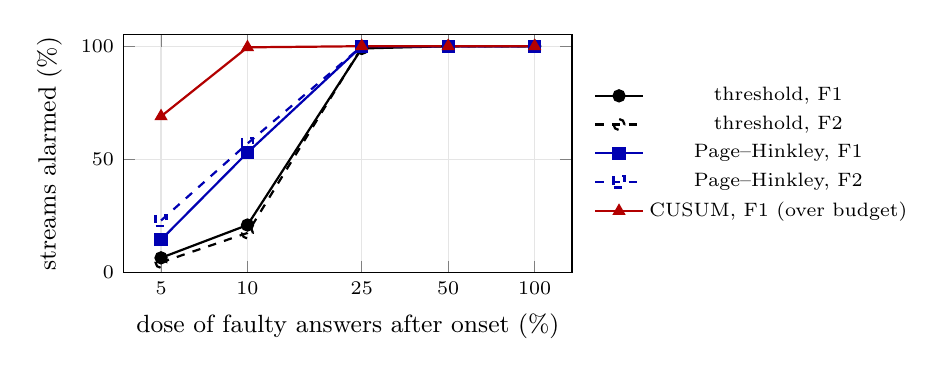
\begin{tikzpicture}
    \begin{axis}[
      width=0.6\textwidth, height=4.6cm,
      xlabel={dose of faulty answers after onset (\%)},
      ylabel={streams alarmed (\%)},
      xmode=log, log basis x=10,
      xtick={5,10,25,50,100}, xticklabels={5,10,25,50,100},
      ymin=0, ymax=105, grid=major, grid style={gray!20},
      legend style={font=\scriptsize, at={(1.03,0.5)}, anchor=west, draw=none},
      tick label style={font=\scriptsize}, label style={font=\small},
    ]
      \addplot[mark=*, thick, black] coordinates {(5,6.5) (10,21.0) (25,99.0) (50,100) (100,100)};
      \addlegendentry{threshold, F1}
      \addplot[mark=o, thick, black, dashed] coordinates {(5,4.5) (10,17.5) (25,99.5) (50,100) (100,100)};
      \addlegendentry{threshold, F2}
      \addplot[mark=square*, thick, blue!70!black] coordinates {(5,14.5) (10,53.0) (25,100) (50,100) (100,100)};
      \addlegendentry{Page--Hinkley, F1}
      \addplot[mark=square, thick, blue!70!black, dashed] coordinates {(5,23.0) (10,57.0) (25,100) (50,100) (100,100)};
      \addlegendentry{Page--Hinkley, F2}
      \addplot[mark=triangle*, thick, red!70!black] coordinates {(5,69.0) (10,99.5) (25,100) (50,100) (100,100)};
      \addlegendentry{CUSUM, F1 (over budget)}
    \end{axis}
  \end{tikzpicture}
  \caption{Detection versus dose under \vthree{} (200 streams of 60 windows per
  point). Threshold points use the sensitivity runs at $W=200$; sequential points
  use the same statistics. CUSUM's high detection comes with pre-onset false
  alarms 3--6 times the budget and 17.5\% alarms on the fresh-seed control.}
  \label{fig:dose}
\end{figure*}

\section{From alarm to action}
\label{app:triage}
Every alarm recorded in the main replays (200 streams per condition) is followed
up in two ways, with the design fixed before either was run. The \emph{readout}
compares the condition's answers with the reference model's answers to the same
questions, using every sample: the change in mean length, in mean agreement among
the $k=4$ samples (S3's measure), and in parse failures. It reads no label. F4 and
F6 reuse healthy answers, so their readout is zero by construction; re-asking the
reference model would give fresh samples, whose change F7 measures (length within
0.3\%, agreement within 0.003). The \emph{check} draws $n$ questions per alarm,
seeded by the stream, from the gradeable slices (\textsf{gsm8k}, \textsf{triviaqa},
\textsf{squad2}, \textsf{banking77}), grades sample 0 of both models, and applies
an exact two-sided McNemar test at $\alpha=0.05$: harm, improvement or no clear
change. Table~\ref{tab:triage} gives \vthree{}'s alarms and the counts for
\vone{} on the harmless shifts. Across all 2{,}868 alarms under \vone{} and \vthree{}, at
both $n$, the check never returned the wrong direction: no harm verdict on U1, F4, F6, F7 or Q1, and no
improvement verdict on a fault.

\begin{table*}[h]
  \centering\small
  \caption{Readout and check after each alarm, \vthree{}. Length and agreement:
  change against the reference model on the same questions (no labels). Accuracy:
  change on all gradeable fault questions, sample 0, with the paired McNemar $p$.
  Check: harm\,/\,improvement verdicts among the alarms when $n$ graded pairs are
  read per alarm. Top: local study; bottom: hosted API.}
  \label{tab:triage}
  \begin{tabular}{lrrrrrcc}
    \toprule
    condition & alarms & length & agreement & accuracy & $p$ & check $n{=}50$ & check $n{=}100$ \\
    \midrule
    F1 & 198 & $-4.0\%$ & $-0.088$ & $-19.1$ & $9\cdot10^{-30}$ & 152\,/\,0 & 194\,/\,0 \\
    F2 & 197 & $-9.2\%$ & $-0.122$ & $-11.2$ & $10^{-16}$ & 71\,/\,0 & 167\,/\,0 \\
    F3 & 199 & $-71.0\%$ & $-0.003$ & $-3.5$ & $7\cdot10^{-5}$ & 3\,/\,0 & 16\,/\,0 \\
    F5 & 191 & $-17.8\%$ & $-0.016$ & $-4.7$ & $3\cdot10^{-4}$ & 13\,/\,0 & 32\,/\,0 \\
    F4 (\vone{}: 196) & 7 & $0$ & $0$ & $0$ & 1 & 0\,/\,0 & 0\,/\,0 \\
    F6 (\vone{}: 200) & 37 & $0$ & $0$ & $0$ & 1 & 0\,/\,0 & 0\,/\,0 \\
    F7 & 0 & $-0.1\%$ & $-0.001$ & $-0.8$ & 0.2 & -- & -- \\
    \midrule
    U1 & 187 & $-7.5\%$ & $+0.043$ & $+4.9$ & $8\cdot10^{-5}$ & 0\,/\,10 & 0\,/\,37 \\
    Q1 & 2 & $-0.1\%$ & $+0.006$ & $+0.1$ & 1 & 0\,/\,0 & 0\,/\,0 \\
    F7 & 3 & $+0.3\%$ & $+0.003$ & $+0.5$ & 0.7 & 0\,/\,0 & 0\,/\,0 \\
    F4 (\vone{}: 198) & 17 & $0$ & $0$ & $0$ & 1 & 0\,/\,0 & 0\,/\,0 \\
    F6 (\vone{}: 200) & 58 & $0$ & $0$ & $0$ & 1 & 0\,/\,0 & 0\,/\,0 \\
    \bottomrule
  \end{tabular}
\end{table*}

\section{Real user traffic}
\label{app:chat}
Every stream in the main text mixes seven benchmark tasks in fixed proportions. A
second pre-registered study, committed before its source was downloaded, replaces
them with real user requests: the first user turns of conversations in one pinned
shard of WildChat-1M~\citep{zhao2024wildchat}, kept only when English, not marked
toxic, redacted or flagged by the logged moderation result, 20--2{,}000 characters
long, and one per repeated template (17{,}460 passed). From these, 3{,}000 were
drawn and split 1{,}500 calibration, 600 held-out and 900 fault; only the prompt
text was kept. The deployment, the update and generation are those of
\S\ref{sec:api}: V4 Flash 0731 as healthy, the same model on fresh seeds (F7) and
V4.1 Flash 1017 (U1). Real traffic has no task labels, so the whole stream is one
slice and pooled and per-slice scoring coincide; S6 reads only intent labels and
was left out ($m=4$). Thresholds were frozen on the healthy calibration answers
before any F7 or U1 answer existed. The 19{,}200 answers cost \$1.85.

\begin{table*}[h]
  \centering\small
  \caption{Real user traffic: 200 replayed streams per condition against the
  frozen record. Signal columns: streams each signal alone detects.}
  \label{tab:chat}
  \begin{tabular}{lrrrrr}
    \toprule
    condition & detected (95\%) & latency & S7 & S1 & S3, S4 \\
    \midrule
    U1 (update) & 89.0\% (83.9--92.6) & 3 & 88.5\% & 63.0\% & 0\% \\
    F7 (fresh seeds) & 4.5\% (2.4--8.3) & 9 & 3.5\% & 0\% & $\le$1\% \\
    \bottomrule
  \end{tabular}
\end{table*}

Table~\ref{tab:chat} gives the result. The update is caught in 89.0\% of streams,
close to the 93.5\% on benchmark traffic, but by S7 rather than S1: 62\% of healthy
chat answers run into the 512-token limit (50\% of the update's), which flattens the
length distribution S1 compares. The held-out windows raise no alarm (nine windows),
and pre-onset false alarms are 0.121\% (95\% interval 0.069--0.211\%), at the
budget as in \S\ref{sec:api}. F7 alarms in 4.5\% of streams, above the 1.8\% that this per-window rate predicts
over its 15 post-onset windows on average: the host does not reproduce seeds
exactly, so fresh-seed answers differ slightly from the calibrated ones (S7 fires
in 3.5\%). The readout of
Appendix~\ref{app:triage} points the same way as on benchmark traffic: under the
update answers are 6.7\% shorter and agreement between samples rises by 0.033
($-7.5\%$ and $+0.043$ there), while F7 moves neither. One slice means this study
cannot test harmless topic shifts, the failure that per-slice scoring fixes.

\section{Datasets and licences}
\label{app:data}
Every source is loaded from the Hugging Face Hub at a pinned revision, and only
the fields listed are read. We release code that rebuilds the questions from these
revisions, not the questions or answers themselves, so no source text is
redistributed. Three sources declare no licence; we use them, as their authors
released them, for non-commercial research only.

\begin{table*}[h]
  \centering\small
  \caption{Sources, the licence each dataset card declares, and what we use.}
  \label{tab:data}
  \begin{tabular}{llll}
    \toprule
    slice & source & licence & used \\
    \midrule
    \textsf{gsm8k} & \texttt{openai/gsm8k} (test) & MIT & question, answer \\
    \textsf{triviaqa} & \texttt{mandarjoshi/trivia\_qa} (rc.nocontext) & none declared$^a$ & question, aliases \\
    \textsf{squad2} & \texttt{rajpurkar/squad\_v2} (validation) & CC BY-SA 4.0 & passage, question, answer \\
    \textsf{banking77} & \texttt{legacy-datasets/banking77} (test) & CC BY 4.0 & query, intent \\
    \textsf{xsum} & \texttt{EdinburghNLP/xsum} (test) & none declared$^b$ & article \\
    \textsf{eli5} & \texttt{sentence-transformers/eli5} & none declared$^c$ & question \\
    \textsf{jsonx} & synthesised by us & -- & -- \\
    chat (App.~\ref{app:chat}) & \texttt{allenai/WildChat-1M}, one shard & ODC-BY & first user turn \\
    \bottomrule
  \end{tabular}\\[2pt]
  {\footnotesize $^a$The card states that the University of Washington does not own
  the copyright of the questions and documents. $^b$BBC news articles.
  $^c$Questions from the r/explainlikeimfive subreddit.}
\end{table*}

\section{Compute and software}
\label{app:compute}
\paragraph{Models} Healthy local model \texttt{gemma4:26b-a4b} (25.8B parameters,
mixture of experts, about 4B active); faults \texttt{gemma4:e2b} (4.6B, about 2B
effective), \texttt{gemma4:e4b} (8.0B, about 4B effective) and \texttt{gemma3:12b}
(12.2B); transfer deployments \texttt{qwen2.5:14b} (14.8B), \texttt{llama3.1:8b}
(8.0B) and \texttt{phi4:14b} (14.7B); judges Qwen 2.5 at 14.8B and 72B; embeddings
Nomic Embed v1.5 (137M). All local models are Q4\_K\_M builds pinned by digest. The
hosted DeepSeek models are identified by version, host and precision
(\S\ref{sec:api}); their size is not stated by the host.

\paragraph{Compute} Every local run used one laptop (Apple M5 Pro, 48\,GB unified
memory) with Ollama 0.40.3. Generating the 64{,}000 main answers took about 31
hours of wall-clock time (healthy 11.0, each fault round 1.5--5.3, the second
healthy model 6.3); the three transfer rounds took at most 162 hours, a span that
includes interruptions. The 14B judge took about 4.5 hours and embedding a few
minutes per round. Hosted generation took about 8 hours (API study 4.8, real
traffic 3.2), and all hosted work, the 72B judge included, cost about \$10.

\paragraph{Settings and software} No hyperparameter was searched. Decoding ($k=4$,
temperature 0.7, at most 512 tokens), windows ($W=200$, $S=50$), the budget
($\beta=0.1\%$) and the bootstrap (20{,}000 windows, generalised Pareto tail) were
fixed before calibration; Appendix~\ref{app:sens} varies the calibration size and
$W$ afterwards. Analyses use Python 3.11 with NumPy 2.4.6, SciPy 1.17.1, pandas
3.0.5, PyArrow 25.0.1 and Hugging Face Datasets 5.0.1; the released lock file pins
every dependency.

\section{Half-sample intervals}
\label{app:half}
\begin{table*}[h]
  \centering\small
  \caption{\vthree{}: Wilson intervals (replay noise only) against intervals from 50
  stratified half-samples of the fault questions (question sampling and replay
  noise). The pre-onset rate here pools the F1--F7 streams; with F4 and F6 it is
  0.017\%.}
  \begin{tabular}{lrcc}
    \toprule
    measure & full data & Wilson 95\% & half-sample 95\% \\
    \midrule
    F1 & 99.0\% & 96--100\% & 96.9--100\% \\
    F2 & 98.5\% & 96--99\% & 96.4--100\% \\
    F3 & 99.5\% & 97--100\% & 98.5--100\% \\
    F5 & 95.5\% & 92--98\% & 92.7--98.3\% \\
    F7 & 0.0\% & 0--2\% & 0.0--1.8\% \\
    pre-onset false alarms & 0.016\% & -- & 0.000--0.061\% \\
    \bottomrule
  \end{tabular}
\end{table*}

\section{Calibration and window size}
\label{app:sens}
\begin{table*}[h]
  \centering\small
  \caption{\vthree{} recalibrated on a share of the calibration questions (ranges over
  three draws per share) and at three window sizes. Runs alarmed
  out of 200.}
  \setlength{\tabcolsep}{4pt}
  \begin{tabular}{lrrrrrrrr}
    \toprule
    setting & threshold change & F1 & F2 & F3 & F4 & F5 & F6 & pre-onset \\
    \midrule
    25\% calib (627 q.) & 14.9--23.0\% & 197 & 195--197 & 199--200 & 10--69 & 192--196 & 118--175 & 0.1--2.1\% \\
    50\% calib (1{,}250 q.) & 4.4--8.2\% & 197--198 & 197 & 197--199 & 9--22 & 191--192 & 35--110 & 0.1--0.2\% \\
    75\% calib (1{,}873 q.) & 4.1--5.4\% & 198 & 197 & 199--200 & 5--9 & 191--192 & 44--60 & 0.0--0.1\% \\
    100\% calib (2{,}500 q.) & -- & 198 & 197 & 199 & 7 & 191 & 37 & 0.0\% \\
    \midrule
    $W=100$ & & 198 & 197 & 200 & 18 & 195 & 94 & 0.1\% \\
    $W=200$ & & 198 & 197 & 199 & 7 & 191 & 37 & 0.0\% \\
    $W=400$ & & 197 & 195 & 194 & 7 & 183 & 17 & 0.1\% \\
    \bottomrule
  \end{tabular}
\end{table*}

\section{Faults on one slice}
\begin{table*}[h]
  \centering\small
  \caption{\vthree{}: runs alarmed (\%) when only one slice is answered by the
  faulty model after the onset. In brackets: accuracy drop in points on that slice.}
  \begin{tabular}{lrrrrrrr}
    \toprule
    fault & gsm8k & triviaqa & squad2 & banking77 & xsum & eli5 & jsonx \\
    \midrule
    F1 & 91.0 (14.4) & 47.5 (24.5) & 66.5 (28.2) & 0.5 (5.0) & 32.0 & 96.5 & 2.0 \\
    F2 & 86.0 (7.5) & 78.0 (15.1) & 34.0 (10.6) & 2.5 (9.7) & 85.0 & 95.0 & 1.0 \\
    F5 & 50.5 (6.0) & 0.5 (0.8) & 2.0 (8.1) & 1.5 (1.5) & 0.5 & 96.5 & 3.5 \\
    \bottomrule
  \end{tabular}
\end{table*}

\clearpage
\section{Judge grades per slice}
\label{app:judge}
\begin{table*}[h]
  \centering\small
  \caption{Mean judge grade (1--10) of the healthy model's answers to the fault
  questions, and each condition's change from it on the same questions. Red: the
  judge grades the condition lower; blue: higher. F3 changes style; F1, F2 and F5
  are weaker models; F7 is the healthy model on fresh seeds.}
  \begin{tabular}{lrrrrrr}
    \toprule
    slice & healthy & F1 & F2 & F3 & F5 & F7 \\
    \midrule
    \textsf{gsm8k} & 8.52 & \cellcolor{blue!4}$+0.13$ & \cellcolor{blue!6}$+0.17$ & \cellcolor{red!26}$-0.77$ & \cellcolor{blue!6}$+0.18$ & $+0.01$ \\
    \textsf{triviaqa} & 7.43 & \cellcolor{red!56}$-1.68$ & \cellcolor{red!26}$-0.77$ & $-0.01$ & \cellcolor{blue!9}$+0.26$ & $-0.02$ \\
    \textsf{squad2} & 6.61 & \cellcolor{red!18}$-0.54$ & $-0.07$ & \cellcolor{blue!6}$+0.19$ & \cellcolor{blue!4}$+0.12$ & $+0.00$ \\
    \textsf{banking77} & 8.06 & \cellcolor{red!11}$-0.32$ & \cellcolor{red!10}$-0.30$ & $-0.05$ & \cellcolor{red!4}$-0.11$ & $-0.01$ \\
    \textsf{xsum} & 7.93 & \cellcolor{red!11}$-0.33$ & \cellcolor{red!3}$-0.09$ & \cellcolor{red!4}$-0.12$ & $+0.04$ & $+0.01$ \\
    \textsf{eli5} & 7.99 & \cellcolor{red!8}$-0.23$ & \cellcolor{red!3}$-0.08$ & \cellcolor{red!60}$-1.80$ & $-0.06$ & $+0.01$ \\
    \textsf{jsonx} & 8.08 & \cellcolor{red!11}$-0.32$ & \cellcolor{blue!3}$+0.09$ & \cellcolor{red!9}$-0.28$ & \cellcolor{red!22}$-0.67$ & $+0.00$ \\
    \midrule
    all & 7.79 & \cellcolor{red!15}$-0.46$ & \cellcolor{red!5}$-0.16$ & \cellcolor{red!17}$-0.52$ & $+0.04$ & $+0.00$ \\
    \bottomrule
  \end{tabular}
\end{table*}

\end{document}
